\chapter{Conclusion and Future Scope}
\label{chapter9}

\section{Conclusion}
The aim of this thesis work as mentioned in the introduction where to investigate and develop a viable method for NoC partitioning, its interfacing with a suitable Quasi-SERDES link interface and implementation on multi FPGA platforms. We simulated, implemented and compared results of different partitioning on Mesh type NoC. Python scripts to automated the process of partitioning NoC with Quasi-SERDES link interface instantiation were used. Simulation results have promising performance. This module was compared with High speed serial IP core provided by Xilinx ``Aurora 8B10B". Both the interfaces have their own advantages and limitations. The Quasi-SERDES link interface module works but has not been optimized in regard to hardware resource utilization and data rates. The python script developed for partitioning has been tested for partitioning mesh type NoC of different dimensions. The script has to be developed further to make it more generalized for any number of router, any configuration type of NoC, any number of partitioning cuts. An other extension to the work was the Raspberry Pi-FPGA integration for Hardware/Software co-design application. Integrating all the work together i.e. Raspberry Pi-FPGA for hardware software co-design and NoC for application independent communication platform will give a systems that can be used for variety of applications exploring and exploiting both sequential and concurrent approach of solving significant problems.

\section{Future Scope}
To carry forward the work a based on the results of this experimentation I can suggest development of dedicated hardware unit to interface DE0 Nano's GPIO pins for multi FPGA network of chips. Considering the example taken earlier in this thesis of 7 $\times$ 7 PG-LDPC where a total of 14 routers are in use in a 4 $\times$ 4 mesh NoC, we shall test similar application on and absolutely dis-integrated NoC in which all the routers are implemented on separate FPGA and the hardware unit supports the high speed interconnection using the Quasi-SERDES link module which is also discussed in chapter 5. A few hardware design considerations while designing the PCB for intergeneration of multiple FPGA units are given below:
\begin{enumerate}
	\item{For high speed communications between two or multiple FPGAs its very important to have the track in between isolated from picking up unwanted interference. To do that its a good practice to provide ground planes and ensuring the beside each high frequency signal carrying track there is a ground line running with it.}
	\item{Termination capacitors should be properly places with the reference guide provided in the device data-sheet.}
	\item{As far as possible to obtain layout and signal integrity, matched and short traces should be used.}
	\item{If you're trying to maximise bandwidth by bundling lots of IO onto a wide parallel bus you may have difficulty keeping all the bits synchronous and without some form of calibration this will drastically reduce the frequency. For example on Cyclone IV you can adjust the output delay from 0 to 150 ps in 50 ps increments but be aware that these values aren't always changeable at run-time so check the data-sheet carefully. Length matching is also an important method to prevent data skewing.}
	\item{You'll almost certainly want to use a source synchronous clocking ( it refers to the technique of having the transmitting device send a clock signal along with the data signals) architecture rather than sharing an external clock. This is also known as globally synchronous local asynchronous (GALS). This will affect your choice of pins.}
	\item{When designing a platform for multi FPGA network of chips its a good idea to make the design modular and repeatable. That is each of the modules and interconnection should be identical so that the FPGA can be chained for any length. To do that the simplest strategy is to map the FPGA interconnection pin to pin. }
\end{enumerate}

The figure \ref{MultiFPGANoC} below tries to give a visual block schematic of the architecture of a modularized PCB design of multi FPGA placement scheme.\\

In this block schematic which has 4 $\times$ 4 FPGA each connect such that each side matches the side of interfaced FPGA. In the Figure \ref{MultiFPGANoC} all the blocks in white are placed on top layer and the black blocks that are shown mirrored are placed on the bottom layer of a multi layered PCB. This chess board design strategy will provide minimum trace lengths, pin to pin mapped design which is repeatable and can be used to develop n $\times$ n FPGA mesh.  This design along with being a modularized and a repeatable design will be neat and easy to assemble and debug. 


\begin{figure} [H]
  \centering
   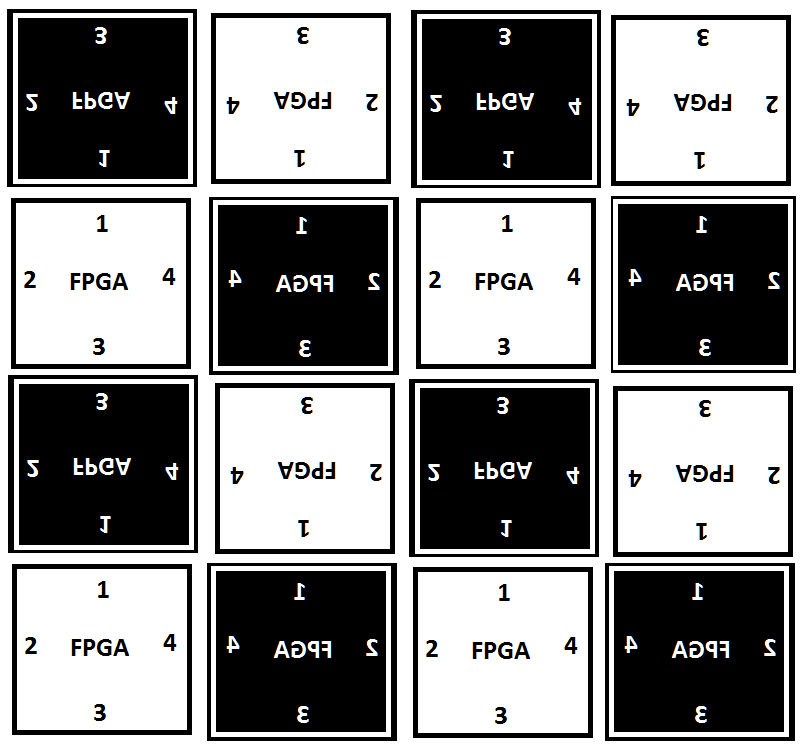
\includegraphics[scale=0.5]{./figs/MultiFPGANoC}
  \caption{Block Schematic of Multi FPGA Network of Chips placement for modular and repeatable design.}
  \label{MultiFPGANoC}
\end{figure}

The figure \ref{BasicPCB} below demonstrates PCB design of each FPGA block in figure \ref{MultiFPGANoC}. This single FPGA design and a supporting interconnect network design can create any topology of multi FPGA network-of-chips.
\begin{figure} [H]
  \centering
   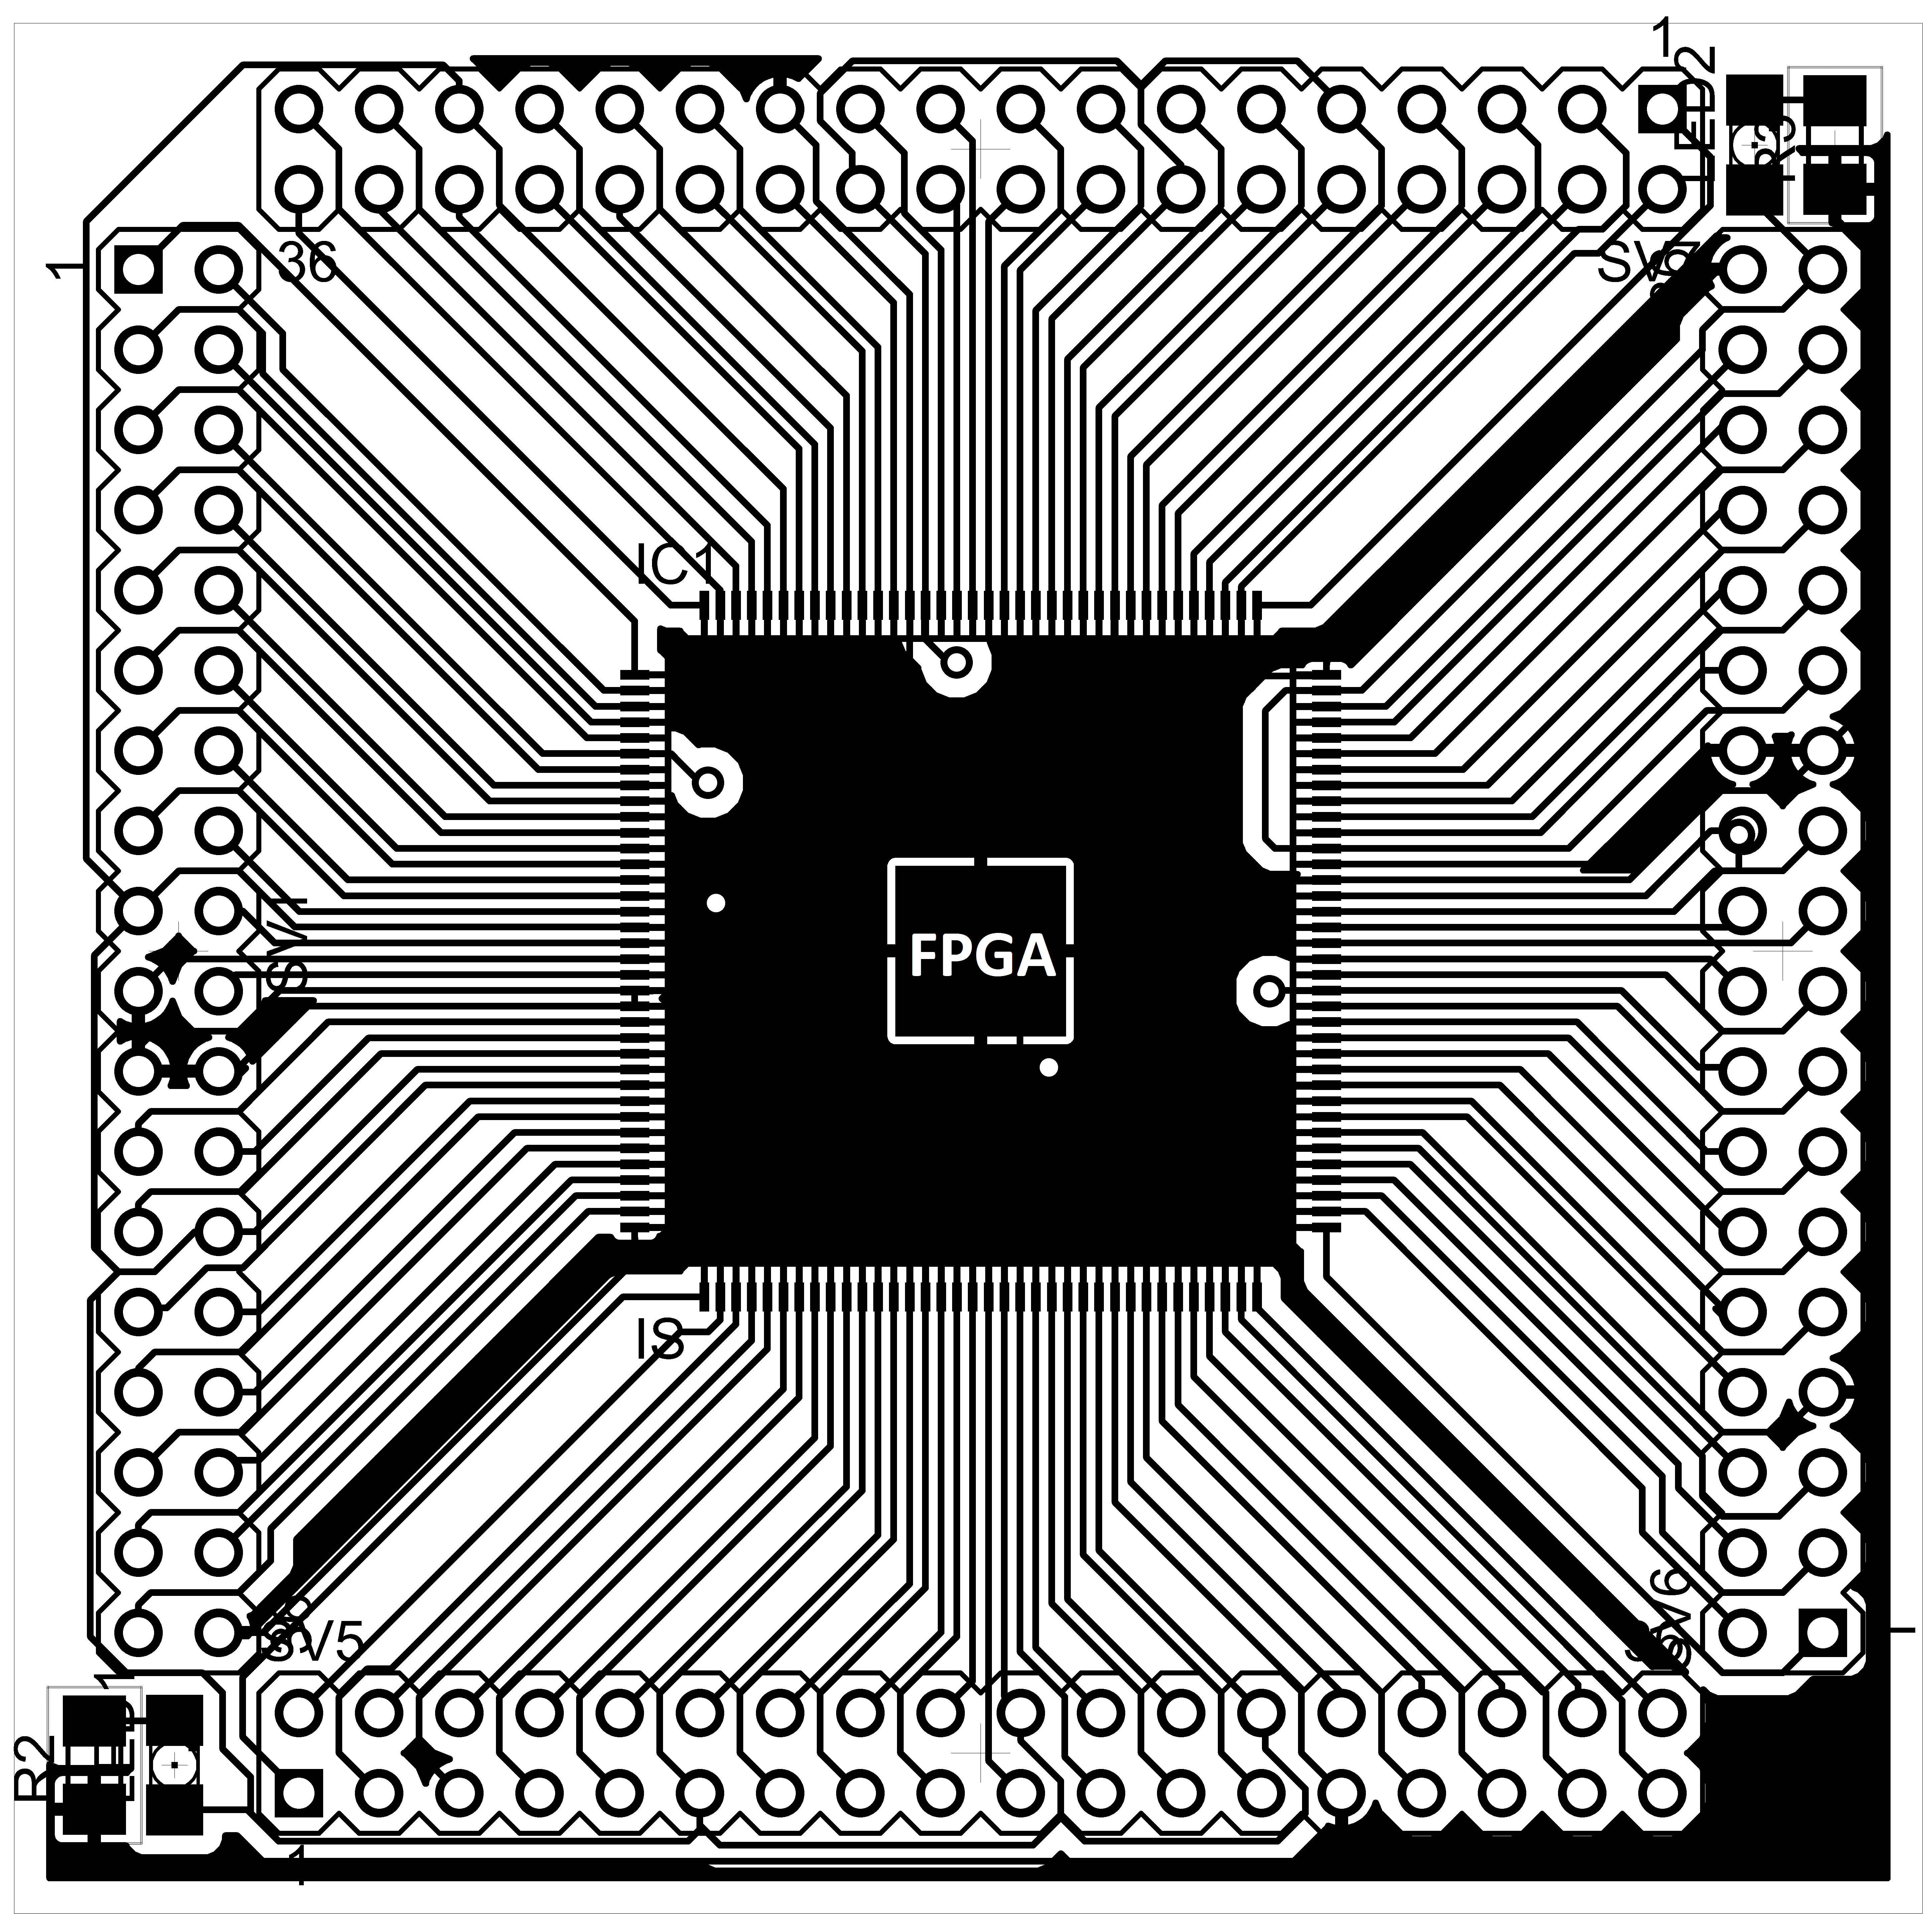
\includegraphics[scale=1.3]{./figs/BasicPCB}
  \caption{Demo PCB Design of each FPGA Block in above figure.}
  \label{BasicPCB}
\end{figure}

